\chapter{Cloud}
Quelle: Wikipedia
\section{Allgemein}
Unter Cloud Computing (deutsch etwa Rechnen in der Wolke) versteht man das Speichern von Daten in einem entfernten Rechenzentrum, aber auch die Ausführung von Programmen, die nicht auf dem lokalen Arbeitsplatzcomputer oder Server installiert sind, sondern eben entfernt in der (metaphorischen) Wolke (englisch cloud).\\\\
Technischer formuliert umschreibt das Cloud Computing den Ansatz, abstrahierte IT-Infrastrukturen (z. B. Rechenkapazität, Datenspeicher, Netzwerkkapazitäten oder auch fertige Software) dynamisch an den Bedarf angepasst über ein Netzwerk zur Verfügung zu stellen. Aus Nutzersicht scheint die zur Verfügung gestellte abstrahierte IT-Infrastruktur fern und undurchsichtig, wie von einer „Wolke“ verhüllt. Angebot und Nutzung dieser Dienstleistungen erfolgen dabei ausschließlich über definierte technische Schnittstellen und Protokolle sowie über lokale Browserfunktionen.\\\\
\textbf{(Geschichte:}Bereits Anfang der 1990er Jahre prophezeiten einige Persönlichkeiten der IT-Branche, dass sich "Computer auf das Netzwerk verteilen" werden, sprich, dass Cloud Computing entstehen werde, sobald die Technik reif sei. Die Zeit war Ende der 1990er mit der Entwicklung der Multitenant-Architektur gekommen. "Salesforce.com" war 1999 schließlich das erste Internetunternehmen, welches Geschäftsanwendungen über eine "normale Website" anbot - was heute als Cloud Computing bezeichnet wird.\\
Als 2004 das soziale Netzwerk Facebook ins Leben gerufen wurde, gab man dessen Mitgliedern die Möglichkeit Fotos, Videos etc. online zu posten und somit abzuspeichern. Damit machte man die Cloud unabsichtlich zu einem persönlichen Service.\\
Der Begriff Cloud Computing wurde jedoch hauptsächlich durch einige schnell wachsende Internetfirmen wie Amazon, Google und Yahoo geprägt. Diese Firmen standen auf Grund des schnellen Wachstums ihrer Nutzerbasis vor dem Problem, ständig wachsende Systeme vorhalten zu müssen, die auch zu Spitzenlastzeiten (für Amazon wäre dies z. B. das Weihnachtsgeschäft) ausreichende Performance bereitstellen.\textbf)

\section{Arten von Clouds}
Es gibt unterschiedliche Arten von Cloud Computing. Eine mögliche Gliederung ist der sogenannte technische Cloud-Stack mit drei Schichten, in der obere Schichten auf den unteren Schichten aufbauen können, es aber nicht müssen:
\begin{enumerate}
\item \textbf{IaaS - Infrastructure as a Service}\\
Die Infrastruktur oder 'Cloud Foundation' stellt die unterste Schicht im Cloud Computing dar. Der Benutzer greift hier auf bestehende Dienste innerhalb des Systems zu, verwaltet seine Recheninstanzen (siehe virtueller Server) allerdings weitestgehend selbst. Dienste innerhalb des IaaS-Konzeptes sind typischerweise verteilte Persistenz (siehe Amazons Simple Storage Service) und ein Nachrichtendienst (siehe Message Oriented Middleware). Sind die Cloud-Dienste selbst noch hochskalierend ausgelegt, trifft dies nicht zwingend auf die Programme zu, die auf den vom Benutzer eingebrachten Recheninstanzen laufen.\\\\
Beispiel: Amazon Web Services
\item \textbf{PaaS - Platform as a Service}\\
Der Entwickler erstellt die Anwendung und lädt diese in die Cloud. Diese kümmert sich dann selbst um die Aufteilung auf die eigentlichen Verarbeitungseinheiten. Im Unterschied zu IaaS hat der Benutzer hier keinen direkten Zugriff auf die Recheninstanzen. Er betreibt auch keine virtuellen Server. Im PaaS-Szenario bringt er ausschließlich seine Programmlogik in die Cloud ein, die ihm gegenüber als Programmierschnittstelle auftritt.

Die Infrastruktur der Cloud selbst kümmert sich hierbei um die erforderliche Instanziierung der Verarbeitungseinheiten und das Verteilen der zu verarbeitenden Daten.\\\\
Beispiel: Windows Azure von Microsoft, 'App Engine' von Google
\item \textbf{SaaS - Software as a Service}\\
Die Anwendungssicht stellt die abstrakteste Sicht auf Cloud-Dienste dar. Hierbei bringt der Benutzer seine Applikation weder in die Cloud ein, noch muss er sich um Skalierbarkeit oder Datenhaltung kümmern. Er nutzt eine bestehende Applikation, die ihm die Cloud nach außen hin anbietet. Dieser Anwendungsfall inkludiert die beiden darunterliegenden Ebenen, da die Cloud-Funktionalitäten wie hochskalierender, verteilter Speicher, ausfallsichere Infrastruktur und üblicherweise ein hochskalierendes Queuingsystem zwar die Grundlage der benutzten Anwendung sind, der Nutzer des SaaS-Dienstes damit allerdings nicht in Kontakt kommt.\\\\
Beispiele: Apple iCloud, Google Drive, Microsoft OneDrive, Dropbox
\end{enumerate}

\section{Zugriff}
Der Zugriff auf die entfernten Systeme erfolgt über ein Netzwerk, beispielsweise das des Internets. Es gibt aber im Kontext von Firmen auch sogenannte 'Private Clouds', bei denen die Bereitstellung über ein firmeninternes Intranet erfolgt. Die meisten Anbieter von Cloudlösungen nutzen die Pooling-Effekte, die aus der gemeinsamen Nutzung von Ressourcen entstehen, für ihr Geschäftsmodell.
\subsection{Arten}
\begin{itemize}
\item \textbf{Public Cloud – die öffentliche Rechnerwolke}
Bietet Zugang zu abstrahierten IT-Infrastrukturen für die breite Öffentlichkeit über das Internet. Public-Cloud-Diensteanbieter erlauben ihren Kunden, IT-Infrastruktur zu mieten auf einer flexiblen Basis des Bezahlens für den tatsächlichen Nutzungsgrad bzw. Verbrauch (pay-as-you-go), ohne Kapital in Rechner- und Datenzentrumsinfrastruktur investieren zu müssen.
\item \textbf{Private Cloud – die private Rechnerwolke}
Bietet Zugang zu abstrahierten IT-Infrastrukturen innerhalb der eigenen Organisation (Behörde, Firma, Verein).
\item \textbf{Hybrid Cloud – die hybride Rechnerwolke}
Bietet kombinierten Zugang zu abstrahierten IT-Infrastrukturen aus den Bereichen von Public Clouds und Private Clouds, nach den Bedürfnissen ihrer Nutzer.
\item \textbf{Community Cloud – die gemeinschaftliche Rechnerwolke}
Bietet Zugang zu abstrahierten IT-Infrastrukturen wie bei der Public Cloud – jedoch für einen kleineren Nutzerkreis, der sich, meist örtlich verteilt, die Kosten teilt (z. B. mehrere städtische Behörden, Universitäten, Betriebe oder Firmen mit ähnlichen Interessen, Forschungsgemeinschaften, Genossenschaften). 
\end{itemize}

\section{Vor- und Nachteile}
Ebenso wie die Virtualisierung ermöglicht Cloud Computing Kostenvorteile gegenüber konventionellen Systemen. Lokale Ressourcen (Software und Hardware) lassen sich einsparen. Vorteile ergeben sich auch im Fall von stark schwankender Nachfrage: Normalerweise müsste man genug Kapazität vorhalten, um Lastspitzen bedienen zu können. Bei Nutzung von Cloud Computing lässt sich die genutzte Kapazität variabel an den tatsächlichen Bedarf kurzfristig anpassen. Dank der Flexibilität und der variablen Skalierbarkeit der Cloud wäre die Bereitstellung benötigter Ressourcen für logistische Software wesentlich günstiger und einfacher zu bewerkstelligen, als es momentan mit statischen Systemen der Fall ist. 

Problematisch stellt sich Datensicherheit beim Cloud Computing dar:

Eines der Grundprobleme, nämlich die Absicherung des Zugriffs auf die Anwendungsdaten beim Transfer zwischen lokalem Client und entferntem Server, kann heute befriedigend gelöst werden. Es existieren zahlreiche Entwicklungen im Bereich der sicheren Übertragung, wie beispielsweise SSL/TLS-Verschlüsselung. Ein weiteres Grundproblem ist die Verschlüsselung der Daten, die in Datenbanken und File-Systemen der Cloud gespeichert werden.
Ein weiteres Problem ist, nämlich dass Administratoren des Cloud-Anbieters und der Dienste Zugriff auf die Nutzerdaten während der Verarbeitung haben, ist hingegen grundsätzlich ohne ein komplexes Management des verteilten Authentisierens und des dynamischen Autorisierens sowie der Kryptografie nicht zu lösen.
Kritiker behaupten, dass die Kontrolle der privaten Daten von Benutzern durch die marktdominanten Anbieter, wie etwa Google, hierdurch überhandnähme. Allerdings gibt es mittlerweile Algorithmen, die Berechnungen so auf einzelne Instanzen aufteilen können, dass es selbst allen Instanzen gemeinsam nicht möglich ist, Rückschlüsse auf die verarbeiteten Daten zu ziehen.Dies ist lediglich der ausführenden Instanz möglich, da nur sie den genauen Algorithmus kennt, mit dem die Teilergebnisse wieder zusammengeführt werden. Ein weiterer Ansatz, der sich zur Behebung dieses Problems eignet, ist die Anwendung einer voll homomorphen Verschlüsselung. Dabei wird innerhalb der Cloud ausschließlich auf verschlüsselten Daten gerechnet, die im privaten Bereich dann wieder entschlüsselt werden können. Die Herausforderung liegt hier jedoch darin, Verschlüsselungsalgorithmen zu finden, die für einen massiven, großflächigen Einsatz beim Cloud Computing effizient genug arbeiten.
Ein alternativer Ansatz, der ebenfalls die Daten in der Cloud unzugänglich macht, ist das Konzept der Sealed Cloud. Dabei kommt eine Schlüsselverteilung zum Einsatz, die zwar eine Verschlüsselung der Daten, jedoch nicht deren Entschlüsselung durch die Schlüssel zulässt, die den Administratoren zugänglich sind, und es erfolgt eine geordnete Sicherung und anschließende Löschung von unverschlüsselten Daten, bevor ein Administrator, beispielsweise zu Wartungszwecken, Zugriff zur Computing-Infrastruktur erhält.
Eine weitere Herausforderung in der Cloud ist die Abhängigkeit (Lock-in-Effekt) vom jeweiligen Cloud-Anbieter, da die angebotenen Schnittstellen meist sehr herstellerspezifisch sind. Privatanwender stehen zudem vor der hypothetischen Frage, was mit ihren Daten in der Cloud passiert, wenn der Anbieter eines Cloud-Dienstes Insolvenz anmeldet. Daher bieten neue Anbieter die Rücksicherung der Daten auf dem eigenen Computer an.


\section{Mögliche Bilder}
\begin{itemize}
\item Bild 1 
\begin{center}
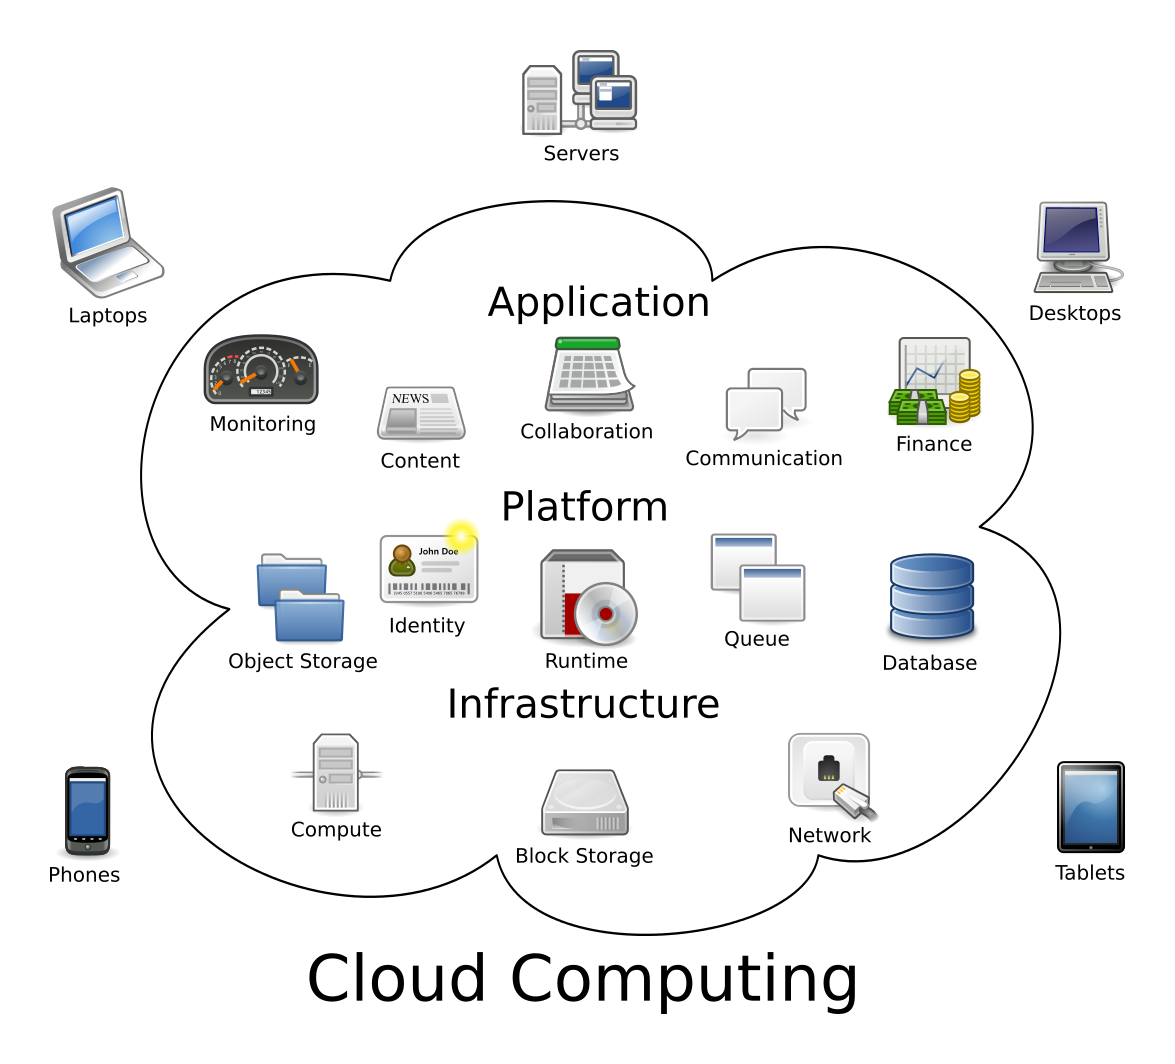
\includegraphics[scale=0.3]{files/img/lyaton_cloud_overview.png}\\
Übersicht\\
\begin{scriptsize}
Quelle: http://de.wikipedia.org/wiki/Cloud\_Computing\#/media/File:Cloud\_computing.svg
\end{scriptsize}
\end{center}
\item Bild 2 
\begin{center}
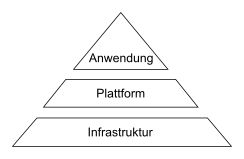
\includegraphics[scale=0.6]{files/img/lyaton_cloud_types.png}\\
Abstraktionsebene von Cloud-Arten\\
\begin{scriptsize}
Quelle: http://de.wikipedia.org/wiki/Cloud\_Computing\#/media/File:Architektur\_Cloud\_Computing.svg
\end{scriptsize}
\end{center}
\end{itemize}

